% 分类目录：dl
\documentclass[12pt]{article}
\usepackage[paperwidth=38cm, paperheight=25cm, margin=1.5cm]{geometry}
\usepackage{ctex}
\usepackage{amsmath, amssymb}
\usepackage{listings}
\usepackage{xcolor}
\usepackage{tabularx}
\usepackage{hyperref}
\usepackage{pgfplots}
\usepackage{longtable}
\usepackage{makecell}
\pgfplotsset{compat=1.18}

% 显著增加表格行高，为图像和公式留足空间
\renewcommand{\arraystretch}{3.5}

\lstset{
    language=Python,
    basicstyle=\ttfamily\tiny,
    keywordstyle=\color{blue},
    commentstyle=\color{green!50!black},
    stringstyle=\color{red},
    showstringspaces=false,
    breaklines=true,
    frame=single
}

\title{核心大矩阵：深度学习激活函数 (Activation Functions) 深度推导与全维度对比}
\author{}
\date{}

\begin{document}
\maketitle

\section{数学推导与设计哲学}
激活函数不仅引入了非线性，还决定了损失曲面的平滑度与梯度流的稳定性。
在近似实现（如 Hard 系列）中，核心设计哲学是**在计算效率与数学拟合度之间取得平衡**。
通常使用泰勒展开（Taylor Expansion）在局部（如 $x=0$）实现高精度拟合，或使用最小二乘法在全局区间（如 $[-3, 3]$）实现工程近似。

\footnotesize
\begin{longtable}{|p{2.2cm}|p{2.8cm}|p{4.5cm}|p{6cm}|p{2cm}|p{2cm}|p{7.5cm}|p{4cm}|}
\hline
\textbf{类别} & \textbf{函数名} & \textbf{公式} & \textbf{深度推导/数学性质 (The Why)} & \textbf{值域} & \textbf{饱和} & \textbf{应用与评价} & \textbf{图像} \\
\hline
\endfirsthead
\hline
\textbf{类别} & \textbf{函数名} & \textbf{公式} & \textbf{深度推导/数学性质 (The Why)} & \textbf{值域} & \textbf{饱和} & \textbf{应用与评价} & \textbf{图像} \\
\hline
\endhead

S型 & Sigmoid & $\frac{1}{1+e^{-x}}$ & \makecell[l]{$f'=f(1-f)$。在 $x=0$ 处的泰勒展开为：\\$\frac{1}{2} + \frac{1}{4}x - \frac{1}{48}x^3 + O(x^5)$。\\其 $1/4$ 是全域最大梯度。} & (0, 1) & 全饱和 & \makecell[l]{二分类输出层标配。由于梯度\\消失，现代深层网络隐藏层已\\少用。} & 
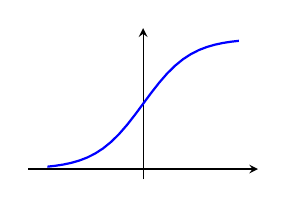
\begin{tikzpicture}[baseline=(current bounding box.center)] 
\begin{axis}[width=4.5cm, height=3.5cm, axis lines=middle, xtick=\empty, ytick=\empty, enlargelimits=true] 
\addplot[blue, thick, domain=-4:4] {1/(1+exp(-x))}; 
\end{axis} 
\end{tikzpicture} \\
\hline

S型 & Tanh & $\frac{e^x-e^{-x}}{e^x+e^{-x}}$ & \makecell[l]{双曲正切。泰勒展开为：\\$x - \frac{1}{3}x^3 + \frac{2}{15}x^5 + \dots$\\在 $0$ 点梯度为 1，比 Sigmoid 响应快。} & (-1, 1) & 全饱和 & \makecell[l]{零中心化特性解决了 Sigmoid\\ 的锯齿形梯度更新问题。} & 
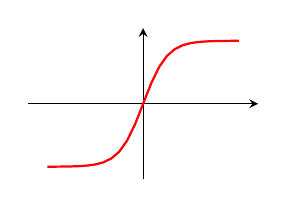
\begin{tikzpicture}[baseline=(current bounding box.center)] 
\begin{axis}[width=4.5cm, height=3.5cm, axis lines=middle, xtick=\empty, ytick=\empty, enlargelimits=true] 
\addplot[red, thick, domain=-4:4] {tanh(x)}; 
\end{axis} 
\end{tikzpicture} \\
\hline

S型 & Hard-Sigmoid & $\begin{cases} 0 & x < -3 \\ \frac{x+3}{6} & [-3, 3] \\ 1 & x > 3 \end{cases}$ & \makecell[l]{\textbf{工程近似}：在 $[-3, 3]$ 区间进行线性拟合。\\虽泰勒展开斜率为 $1/4$，但 $1/6$ 斜率\\在较大区间内能最小化 MSE 误差，且\\对定点化硬件极度友好。} & [0, 1] & 全饱和 & \makecell[l]{MobileNet 等轻量级网络首选。\\牺牲局部精度换取推理速度。} & 
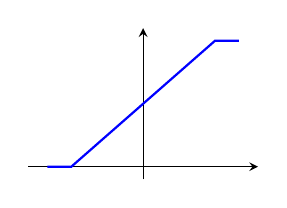
\begin{tikzpicture}[baseline=(current bounding box.center)] 
\begin{axis}[width=4.5cm, height=3.5cm, axis lines=middle, xtick=\empty, ytick=\empty, enlargelimits=true] 
\addplot[blue, thick, domain=-4:4] {max(0, min(1, x/6 + 0.5))}; 
\end{axis} 
\end{tikzpicture} \\
\hline

ReLU族 & ReLU & $\max(0, x)$ & \makecell[l]{一阶导数为阶跃函数。\\本质是单侧抑制。解决了饱和区\\带来的梯度消失问题。} & [0, +$\infty$) & 半饱和 & \makecell[l]{现代深度学习的基石。\\简单、高效、稀疏。} & 
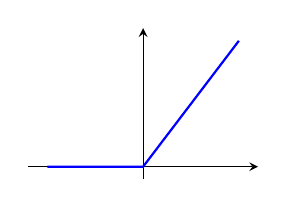
\begin{tikzpicture}[baseline=(current bounding box.center)] 
\begin{axis}[width=4.5cm, height=3.5cm, axis lines=middle, xtick=\empty, ytick=\empty, enlargelimits=true] 
\addplot[blue, thick, domain=-2:2] {max(0, x)}; 
\end{axis} 
\end{tikzpicture} \\
\hline

ReLU族 & Leaky ReLU & $\begin{cases} x & x \ge 0 \\ \alpha x & x < 0 \end{cases}$ & \makecell[l]{泰勒展开在 $x<0$ 无效。\\通过 $\alpha$ 保持负半轴有微弱梯度流，\\属于经验性设计，旨在修复 Dead ReLU。} & (-$\infty$, +$\infty$) & 无 & \makecell[l]{$\alpha$ 通常设为 0.01。\\旨在增加负向激活的稳健性。} & 
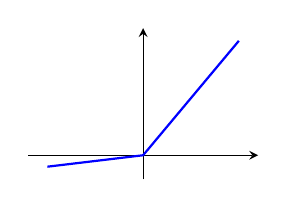
\begin{tikzpicture}[baseline=(current bounding box.center)] 
\begin{axis}[width=4.5cm, height=3.5cm, axis lines=middle, xtick=\empty, ytick=\empty, enlargelimits=true] 
\addplot[blue, thick, domain=-2:2] {x > 0 ? x : 0.1*x}; 
\end{axis} 
\end{tikzpicture} \\
\hline

ReLU族 & PReLU & $\max(\alpha x, x)$ & \makecell[l]{Parametric ReLU。将 $\alpha$ 视为可导变量。\\数学上允许模型根据反向传播\\自适应学习不同层的激活特性。} & (-$\infty$, +$\infty$) & 无 & \makecell[l]{在图像分类竞赛（如 ImageNet）\\中曾大幅提升模型性能。} & 
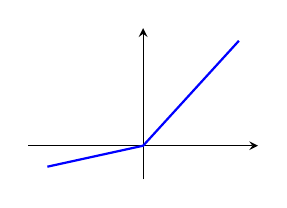
\begin{tikzpicture}[baseline=(current bounding box.center)] 
\begin{axis}[width=4.5cm, height=3.5cm, axis lines=middle, xtick=\empty, ytick=\empty, enlargelimits=true] 
\addplot[blue, thick, domain=-2:2] {x > 0 ? x : 0.2*x}; 
\end{axis} 
\end{tikzpicture} \\
\hline

ReLU族 & ELU & $\begin{cases} x & x \ge 0 \\ \alpha(e^x-1) & x < 0 \end{cases}$ & \makecell[l]{指数线性单元。负半轴具备软饱和性。\\指数项使得均值更接近 0，\\具备自然的“自归一化”特性。} & (-$\alpha$, +$\infty$) & 负向饱和 & \makecell[l]{在噪声较大的任务中具有更好\\ 的鲁棒性。} & 
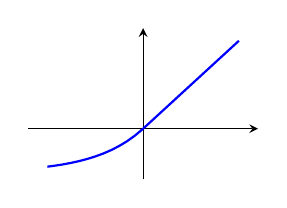
\begin{tikzpicture}[baseline=(current bounding box.center)] 
\begin{axis}[width=4.5cm, height=3.5cm, axis lines=middle, xtick=\empty, ytick=\empty, enlargelimits=true] 
\addplot[blue, thick, domain=-2:2] {x > 0 ? x : (exp(x)-1)}; 
\end{axis} 
\end{tikzpicture} \\
\hline

ReLU族 & Softplus & $\ln(1+e^x)$ & \makecell[l]{ReLU 的解析平滑近似。\\其导数恰好为 Sigmoid 函数：\\$f'(x) = \frac{e^x}{1+e^x} = \sigma(x)$。} & (0, +$\infty$) & 无 & \makecell[l]{多用于变分自编码器 (VAE) \\ 的方差约束预测。} & 
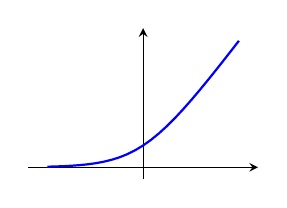
\begin{tikzpicture}[baseline=(current bounding box.center)] 
\begin{axis}[width=4.5cm, height=3.5cm, axis lines=middle, xtick=\empty, ytick=\empty, enlargelimits=true] 
\addplot[blue, thick, domain=-4:4] {ln(1+exp(x))}; 
\end{axis} 
\end{tikzpicture} \\
\hline

现代平滑 & SiLU (Swish) & $\frac{x}{1+e^{-x}}$ & \makecell[l]{\textbf{自门控机制}：$x \cdot \sigma(x)$。\\由 RL 神经网络搜索发现。\\非单调性允许在负值区间保留梯度。} & [-0.28, +$\infty$) & 无 & \makecell[l]{EfficientNet 性能飞跃的关键。\\大模型前馈层（FFN）的基础。} & 
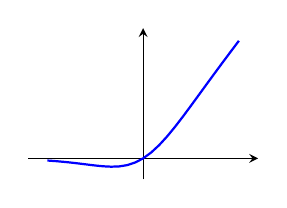
\begin{tikzpicture}[baseline=(current bounding box.center)] 
\begin{axis}[width=4.5cm, height=3.5cm, axis lines=middle, xtick=\empty, ytick=\empty, enlargelimits=true] 
\addplot[blue, thick, domain=-4:4] {x/(1+exp(-x))}; 
\end{axis} 
\end{tikzpicture} \\
\hline

现代平滑 & GELU & $x\Phi(x)$ & \makecell[l]{\textbf{随机性正则}：$x$ 与其分布概率的乘积。\\$\Phi(x)$ 为标准正态分布的 CDF。\\它是 Dropout 与 激活函数的概率融合。} & [-0.17, +$\infty$) & 无 & \makecell[l]{\textbf{LLM 时代的默认选择}。\\BERT、GPT 系列的通用内核。} & 
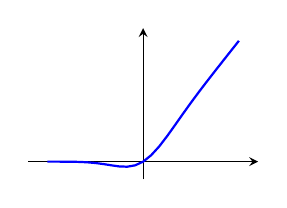
\begin{tikzpicture}[baseline=(current bounding box.center)] 
\begin{axis}[width=4.5cm, height=3.5cm, axis lines=middle, xtick=\empty, ytick=\empty, enlargelimits=true] 
\addplot[blue, thick, domain=-4:4] {0.5*x*(1+tanh(sqrt(2/3.14159)*(x+0.044715*x^3)))}; 
\end{axis} 
\end{tikzpicture} \\
\hline

现代平滑 & Mish & $x\tanh(Softplus)$ & \makecell[l]{\textbf{自正则化非单调性}。\\保持了全阶连续性，比 ReLU 更利于\\梯度反向传播。平滑曲线减少了信息损失。} & [-0.31, +$\infty$) & 无 & \makecell[l]{YOLOv4 等 SOTA 视觉网络。\\训练稳定性优于 ReLU/Swish。} & 
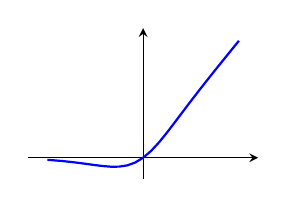
\begin{tikzpicture}[baseline=(current bounding box.center)] 
\begin{axis}[width=4.5cm, height=3.5cm, axis lines=middle, xtick=\empty, ytick=\empty, enlargelimits=true] 
\addplot[blue, thick, domain=-4:4] {x*tanh(ln(1+exp(x)))}; 
\end{axis} 
\end{tikzpicture} \\
\hline

门控回归 & SwiGLU & $Swish(xW) \otimes xV$ & \makecell[l]{GLU (门控线性单元) 的平滑变体。\\通过增加参数量实现更精细的特征筛选。\\本质是高度非线性的动态滤波器。} & (分布式) & 无 & \makecell[l]{\textbf{Llama 3, Qwen 2 等 LLM 标配}。\\针对计算资源丰富场景设计。} & 
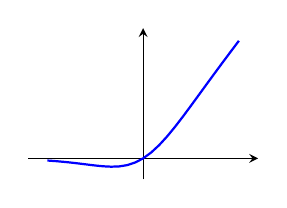
\begin{tikzpicture}[baseline=(current bounding box.center)] 
\begin{axis}[width=4.5cm, height=3.5cm, axis lines=middle, xtick=\empty, ytick=\empty, enlargelimits=true] 
\addplot[blue, thick, domain=-4:4] {x/(1+exp(-x))}; 
\end{axis} 
\end{tikzpicture} \\
\hline

复合型 & Maxout & $\max(w_1^T x, w_2^T x)$ & \makecell[l]{\textbf{分段线性逼近者}。\\可以将任何凸函数局部逼近为多条直线。\\由分层参数决定激活的凸度。} & (-$\infty$, +$\infty$) & 无 & \makecell[l]{参数极多，拟合力强，现多被\\更加高效的门控网络取代。} & 
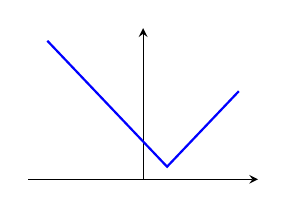
\begin{tikzpicture}[baseline=(current bounding box.center)] 
\begin{axis}[width=4.5cm, height=3.5cm, axis lines=middle, xtick=\empty, ytick=\empty, enlargelimits=true] 
\addplot[blue, thick, domain=-2:2] {max(x, -x+1)}; 
\end{axis} 
\end{tikzpicture} \\
\hline
\pagebreak
\caption{机器学习激活函数深度逻辑与性能矩阵 (百科级版本)}
\end{longtable}

\section{核心代码参考 (PyTorch)}
\begin{lstlisting}
import torch.nn as nn

# 工业级标准选型推荐
class ActivationChoice(nn.Module):
    def __init__(self, task_type='nlp'):
        super().__init__()
        if task_type == 'cv':
            self.act = nn.ReLU() # 视觉默认基准
        elif task_type == 'nlp':
            self.act = nn.GELU() # Transformer/BERT 标准选型
        elif task_type == 'swiglu':
            self.act = nn.SiLU() # Llama, Qwen 等 LLM 前馈层的核心
        else:
            self.act = nn.Mish() # 追求极致精度的 SOTA 视觉方案
\end{lstlisting}

\end{document}
